\section{Approach}
\label{sec:approach}

In this section, we introduce our test prioritization approach in detail. In particular, we first present the overview of our approach, major technical challenges, and our performance model. After that, we introduce performance-impact estimation of a code commit based on our performance model, including method-execution-time estimation, and method-invocation-frequency estimation based on collection-loop correlation and iteration-count inference.


\subsection{Overview}

%To prioritize performance test cases, the core difficult

%The objective of PerfChecker is to examine a code commit content and determine the cost of a change, and then rank the performance test case on basis of a change performance impact cost which helps to reduce the cost in performance regression testing. Profiler takes the base version code and statically modifies the code in order to extract profile information. Run all the performance test case and store method execution time, execution frequency and loop counter in profile database.Profile database also store JDK library method's execution summary. 

\begin{figure}
\centering
	
	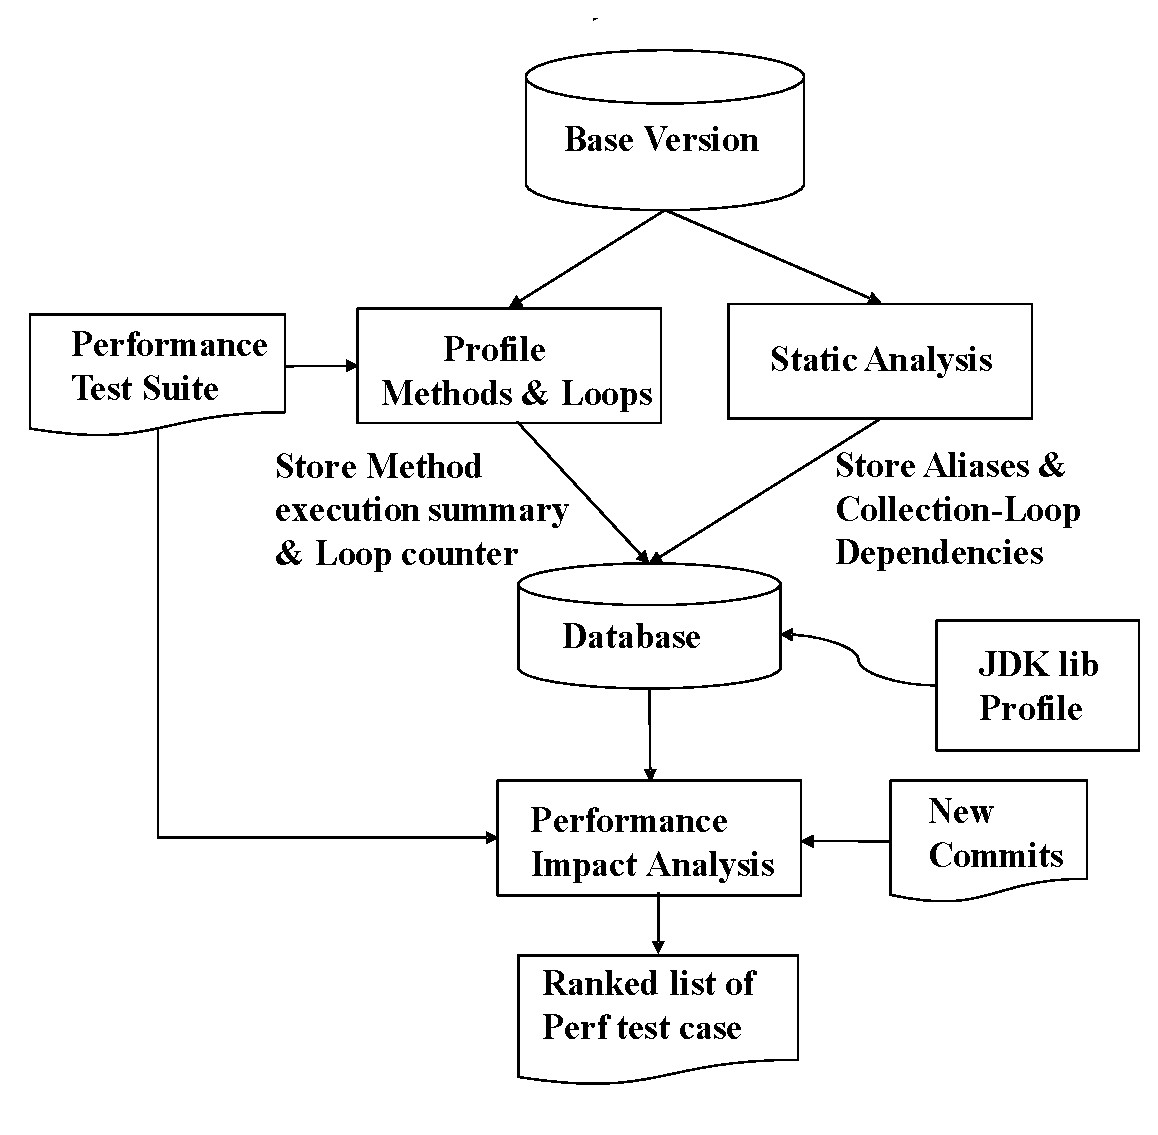
\includegraphics[width=3.5in, height=3.5in]{performance/images/Workflow2.pdf}
	\caption{Workflow of Our Approach}	
	\label{fig:approach-workflow}
		
\end{figure}

Figure~\ref{fig:approach-workflow} shows the workflow of our approach. The input to our approach includes the project code base, its code commits, and performance test cases. The output of our approach is an ordered list of performance test cases. The first step of our approach is to  profile the base version of the project under test. During the profiling, for each test case, we record the dynamic call graph as its original performance model. We also record average execution time and frequency of methods, and iteration counts of all loops. At the same time, we statically analyze the base version to gather dependencies between loops and collection variables, as well as aliases among collection variables. When a new code commit comes, we conduct performance impact analysis to estimate its performance impact on all test cases, and prioritize test cases accordingly. 


%Another component is Alias analyzer which statically analyze the source code loop controlling variable, array and collection with their alias and store their information in database. Diff generator produce diff of each committed code into the repository. Parser parses information regarding the changed files, lines and types (add, delete) from the generated diff file content. Filter prunes out insignificant change such as stylish change or renaming. If the changes are significant, the commit will be considered to fed to the performance impact analyzer. Performance impact analyzer analyse the cost of the change by constructing CFG of the modified method and integrating the profile information from the database into the call graph of the test case. At the final stage it produce a sorted list of test case according the cost performance impact score. 



 
 
%The challenge is how to estimate the cost about performance impact of each of test case after a change without actually running the software.We first briefly describe the input-output of our approach and major component. 

%Although it is straightforward to prioritize test cases based on the code commit's performance impact on them, 

\textbf{Technical Challenges.} Performance impact analysis is the core of our approach. Although we focus on collection-intensive software, it is still challenging to conduct performance impact analysis, facing three major technical challenges:

\begin{itemize}

\item Challenge 1. A code commit may include any type and scope of code changes, from one-line revision, to feature addition and interface revision. Therefore, there is a strong need of a unified and formal presentation for code commits.  

\item Challenge 2. A code commit may contain newly added code, especially new loops. No execution information of such code is available, but given that loops can have high impact on performance, there is a strong need of estimating the code commit's execution time and frequency.
 
\item Challenge 3. Even if the execution time of changed code in a code commit has little impact on performance, the code commit may include changes on collection variables, eventually affecting the performance of unchanged code. 

%In our paper, we refer such performance changes as \textit{side performance impact}. 

\end{itemize}

To address Challenge 1, we present a code commit as three sets of methods: added methods, revised methods, and removed methods. As our performance model is based on the dynamic call graph, any code commit can be mapped to a series of operations for method addition, removal, and replacement in the performance model. To address Challenge 2, we leverage the recorded profiling information of the base version as much as possible. Specifically, if an existing method is invoked in the newly added code, we can use the recorded execution time of the existing method as its execution-time estimation for this new invocation. Furthermore, as discussed in Section~\ref{sec:intro}, we use collection variables as bridges to estimate iteration counts of new loops from those of existing loops. To address Challenge 3, we track all the element-addition and element-removal operations of collection variables in the newly added code, and estimate the size change of collection variables from the iteration count of their enclosing loops. This new size is used to update the iteration counts of loops depending on the changed collection variables. 

%Note that, the execution time of added and removed methods can affect existing test executions only through revised methods, where invocations to them are added and removed. %For each revised method, based on the performance model in Section~\ref{subsec:model}
%we estimate the execution time of the pre-commit version and post-commit version, respectively, and estimate the performance impact of a revised method as the execution-time difference between its pre-commit version and post-commit version. Then, the directly performance impact of a code commit can be calculated as the performance impact sum of all revised methods, together with side performance impact. 



%and if a newly added loop depends on an existing collection variable, 

%we can use the recorded size of the collection variable to estimate the number of iterations of the loop. The detailed process of estimating direct performance impact is presented in Section~\ref{subsec:direct}. 



%their new value ranges in the new version according to the iteration number of the writing operations. Then, for each collection variable $v$, if there is any loop $l$ depending on $v$, we calculate the side performance impact of $l$ with $v$'s new value range and sum up side performance impact of all such loops. The detailed process of estimating side performance impact is presented in Section~\ref{subsec:side}.

Since we focus on collection-intensive software, we consider only loops whose iteration number depends on collection variables, e.g., variables of array type, and other collection types defined in Java Utility Collections. Note that there are also some loops whose iteration number depends on simple integers, such as a loop to sum up a numbers from $i$ to $j$, but such loops are not common in collection-intensive software, and our evaluation results show that our approach is effective on both data-processing software (Xalan) an mathematics software (Apache Commons Maths). 

%The rationale behind this design decision are (1) according to literatures~\cite{}~\cite{}, most performance issues are related to loops; and (2) most loops in programs are for manipulating iterative data structures (i.e., collection variables).  


%This is a limitation of our performance impact analysis, b ut 
  
\subsection{Performance Model}
\label{subsec:model}
\begin{figure}[t]
\centering
  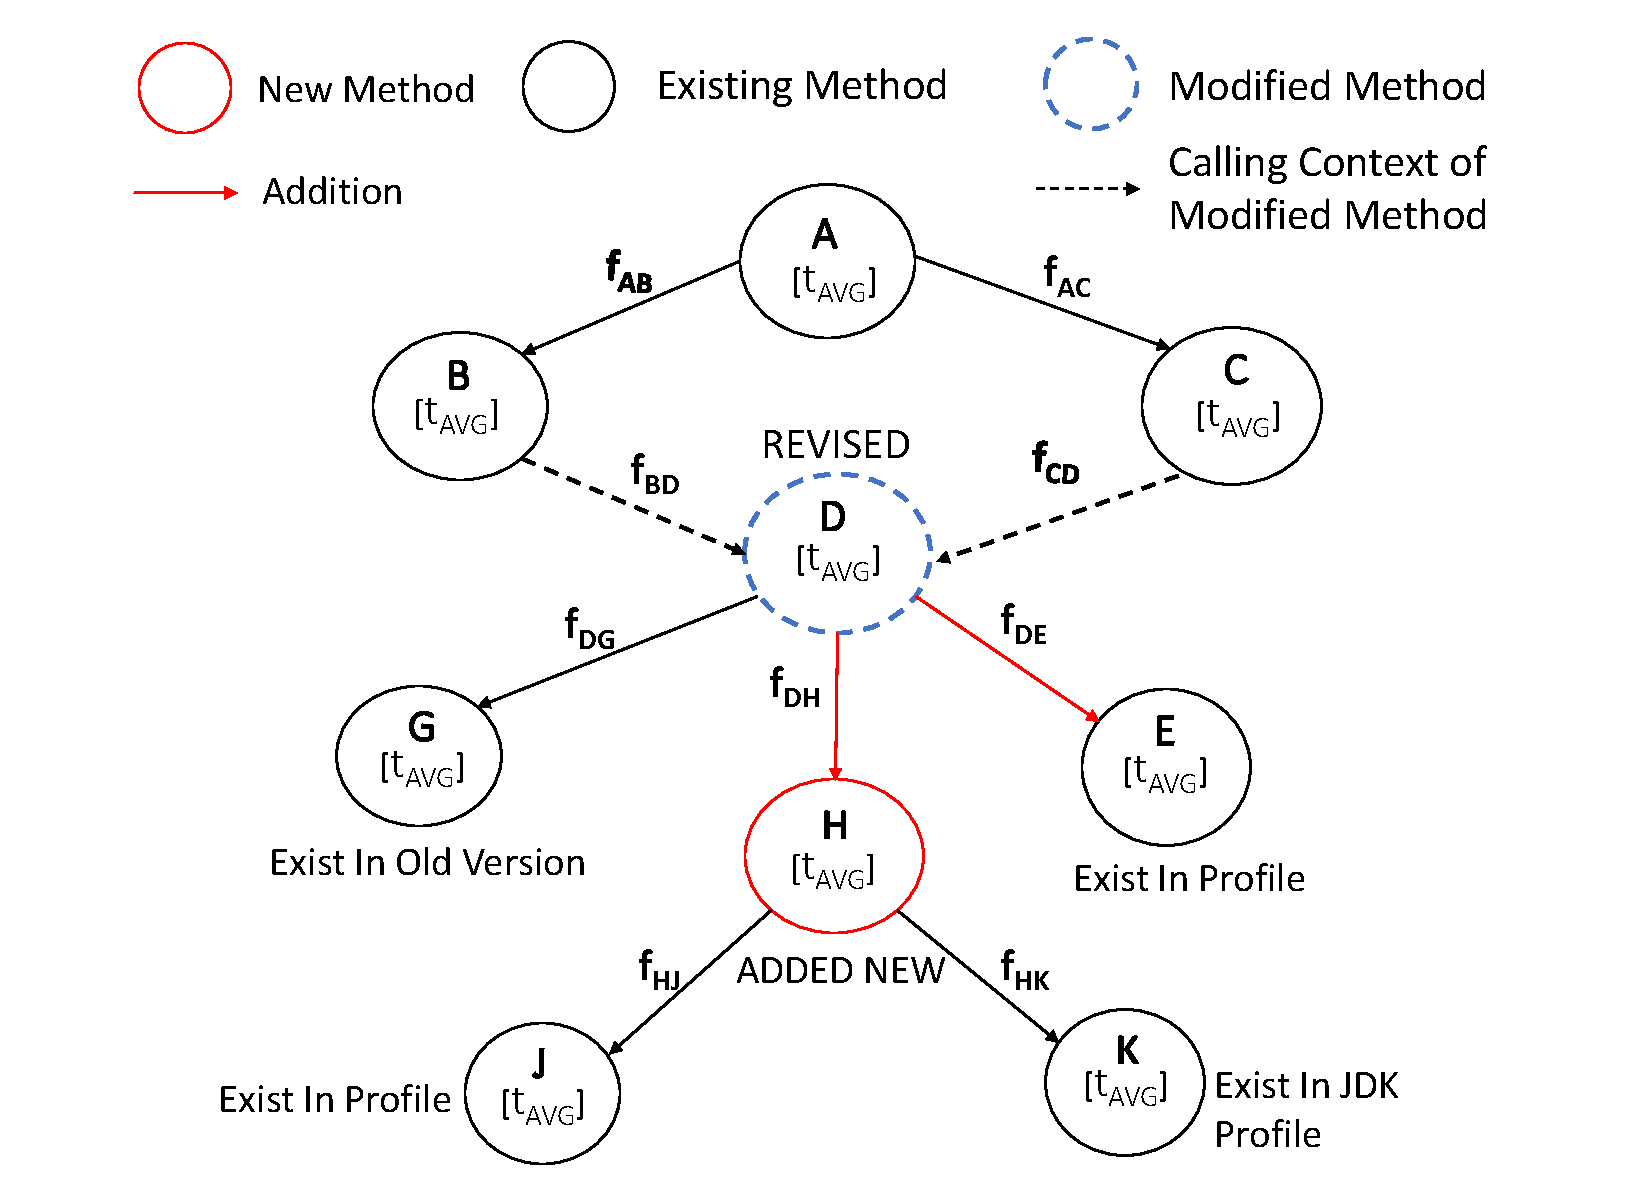
\includegraphics[width=4in, height=3in]{performance/images/performance-model.pdf}
  
   \caption{An Example Performance Model}	
    \label{fig:performance-model}
   
 \end{figure}

In this subsection, we introduce our performance model to break  down execution time of a test case to all the methods invoked by the test case. The basic intuition behind our model is that the execution time of a method invocation $M$ is the execution-time sum of all method invocations directly invoked in $M$, together with the execution time of instructions in $M$. Since most basic operations in Java programs are performed by JDK library methods (e.g., a string concatenation), the latter part is typically trivial compared with the former part, so our performance model ignores instructions in $M$ itself, but focuses only on methods that $M$ invokes. 

%Specifically, for each test case, our performance model is based on the dynamic call graph of the test case. So the nodes of the graph are method bodies, and the edges are invocations. In the graph, we record two attributes: invocation frequency, and average execution time. For example, on the directed edge from method $A$ to method $B$, we record the average number of invocations from $A$ to $B$ in each invocation of $A$, and on the node $B$, we record the average execution time of $B$.  

We illustrate our model in Figure~\ref{fig:performance-model}, where each node represents a method and each directed edge represents an invocation relation. Here each node annotated with label $t_{avg}$, which represents the average execution time of a method. Each edge in the graph is labeled with $f_{AB}$, which represents the invocation frequency of method B from method A. Given a code commit, the performance model of the post-commit version can be acquired by adding and removing nodes and edges to the original performance model. For example, in Figure~\ref{fig:performance-model}, method $D$ is a revised method and it now calls (1) method $G$, which it originally calls, (2) $E$, which is an existing method in the base version, and (3) $H$, which is a newly added method. With the average execution time and invocation frequency of all invoked methods in $D$, we are able to calculate an execution-time estimation for revised method $D$. The new execution time at $D$ can be propagated upward to its ancestors, until the main method is reached and a new estimation of the whole program's execution time can be made. 


% $m\textsubscript{K}$ are changed and they are called from multiple context $m\textsubscript{B}$,$m\textsubscript{G}$  and $m\textsubscript{H}$. So the total cost is calculated from the modification cost of method $m\textsubscript{J}$  and $m\textsubscript{K}$ by multiplying the frequency  $f\textsubscript{BJ}$,$f\textsubscript{GJ}$,$f\textsubscript{HK}$ and $f\textsubscript{GK}$. Finally, The cost is propagated from child to parent in the graph.

\subsection{Performance Impact Analysis}
\label{subsec:direct}

The basic idea of performance impact analysis is to calculate the  execution-time change of each revised method $M$ in the code commit. Then, through propagating the execution-time change to $M$'s predecessors in the performance model, we can calculate the execution-time change of the whole test case at the root node. 

%We focus only on revised methods because added and removed methods may affect software performance only through revised methods (i.e., by adding or removing method invocations).

We realize this idea in three steps. First, for each revised method, we extend the performance model to either add it and/or some of its callees (and transitive callees). Second, we estimate the execution-time change of each method in the new performance model. Third, we estimate the invocation frequency on the edges of the new performance model. We next introduce the three steps in details.



\subsubsection{Model Extension}
\label{subsub:findInvoke}

For each revised method, we add its direct and transitive callees (e.g., methods $E$ through $K$ in Figure~\ref{fig:performance-model} for the revised method $m_D$) into the performance model, if they do not already exist in the model. In this recursive process, we terminate the extension of a method node if it is an unrevised method existing in the base version, a JDK library method, or a method whose source code is not available. Since we use one base version for a series of code commits, a revised method (and even some of its predecessors) may not exist in the base version because they are added after the base version. In such a case, we transitively determine $M$'s predecessors (callers) until we reach methods in the base version. For example, if $C$ and $D$ in Figure~\ref{fig:performance-model} are added between the base version and the code commit under analysis, we determine that $D$ is invoked by $B$ and $C$, and $C$ is invoked by $A$, so that we add $C$ and $D$ to the performance model. 

When the new code version of the revised methods is available, we  
statically determine the direct and transitive callers and callees for the revised method, and one remaining challenge is to resolve polymorphism, where one method invocation may have multiple targeted method bodies. Although it is straightforward to apply off-the-shelf points-to analysis, since we have the profiling information of the base version, we make use of the information to acquire a more precise call graph. Specifically, if a method invocation is not involved in the method diff (i.e., the method invocation can be mapped to the same method invocation in the base version, such as $G$ in Figure~\ref{fig:performance-model}), we assume that its target is not changed and we use the same targeted method body as recorded for the base version. Otherwise, we apply points-to analysis~\cite{Spark} in Soot~\cite{Soot} to find the possible targeted method bodies for the method invocation. When a method invocation is mapped to multiple method bodies, we add all bodies to the new performance model, and we divide the estimated frequency of the method invocation by the number of possible targets to attain the invocation frequency of each target. 

%Analyzing the new code version of the revised method, it is straightforward to build a partial call graph with it as the root node. Since  resolve polymorphism, we use the following heuristic. 

%Therefore, by listing all the added and deleted methods and their execution time summary will provide an estimate of 

%So combining the profiling information and control flow analysis together may provide accurate estimate of cost of modified method.

%Estimate the cost of a modified method need to identify all the changes inside the method which are added and deleted.




\subsubsection{Execution-Time Change of Method Bodies}
\label{subsub:findExetime}

The method bodies invoked from a revised method fall into three  categories. The first category is removed method bodies. Their execution-time data are recorded in the performance model of the base version, and their new execution time is estimated as 0.

The second category includes method bodies already existing in the performance model of the base version. Such method bodies include both those defined in the source code and those defined in the JDK library, or those without source code. For existing method bodies, we simply use the recorded average execution time in the base version as their estimated average execution time. For bodies of JDK library methods, we profile Dacapo~\cite{dacapo} to acquire the average execution time of those common JDK library methods. For methods without source code or those not invoked by Dacapo, we use the average execution time of all method bodies in the profile as their estimated execution time, as we have no further information. Note that when a method from the second category is added to the performance model, its original execution time is set as 0.

The third category includes newly added method bodies in the source code. \textit{Note that such method bodies include both those added to the source code in the code commit and those added in any other code commits between the base version and the code commit under analysis.} They also include method bodies defined in libraries but are newly reached due to code revisions from the base version to the new version. For a newly added method body (such as $H$ in Figure~\ref{fig:performance-model}), as discussed in Section~\ref{subsub:findInvoke}, we extract all its callee method bodies, and add them to the performance model (such as $J$ and $K$ in Figure~\ref{fig:performance-model}), and then we calculate its execution-time change using our performance model.

%If an added callee method body still belongs to category-2, then we can iteratively extract its callee method bodies. The extraction process will terminate when all the newly added callee method body either belongs to category-1, or is defined in Java SDK. 



%Changes inside a method normally consists of addition and deletion of existing method call or addition of newly method call. 
%Profile all the performance test case and store their average execution time  will provide the cost of existing method call.
%A newly added method also consists of existing method, JDK library call and newly added method. So profiling JDK library function call
%also helpful to estimate the cost of newly added method. if no information available then statically analyse the change and assign the cost based on the existence of loop and hot api call like database, storage and network.
 
\subsubsection{Invocation Frequencies of Method Bodies}

Given a newly added or revised method $m_x$, for each method $m_y$ that is directly invoked in $m_x$, we estimate the invocation frequency of $m_y$ in $m_x$ (denoted as $fq(m_x, m_y)$) to apply our performance model on the new version. Our estimation technique is based on the control flow graph of $m_x$ and the average iteration counts of loops in $m_x$. Specifically, for any code block $b$ in $m_x$, we use $fq(b, m_y)$ to denote the invocation frequency of $m_y$ from $b$ for each execution of $b$. If $b$ is a basic block without branches and loops, $fq(b, m_y)$ is exactly the number of invocation statements to $m_y$ in $b$; such number can be easily counted statically. Then we calculate $fq(m_x, m_y)$ by applying the inference rules for sequential, branch, and loop structures in Formulas~\ref{equa:seq}-\ref{equa:loop} below recursively on the code blocks of $m_x$:

   
\begin{equation}
\label{equa:seq}
fq([\text{$b_1$; $b_2$}], m_y) = fq(b_1, m_y) + fq(b_2, m_y)
\end{equation}
\begin{equation}
\label{equa:branch}
fq([\text{if() $b_1$ else $b_2$}], m_y) = Max(fq(b_1, m_y), fq(b_2, m_y))
\end{equation}
\begin{equation}
\label{equa:loop}
fq([\text{while$_i$ () $b$}]) = fq(b, m_y) \times C(loop_i)
\end{equation}

In the inference rules, the only unknown parameter is $C(loop_i)$, which denotes the average iteration count of the i$^{th}$ loop in $A$. As an example, given the control flow graph in Figure~\ref{fig:cfg-sample} of m$_x$, for any $m_y$ that $m_x$ invokes, $fq(m_x, m_y)$ can be estimated as in Formula~\ref{equa:example}.

\begin{figure}
\centering
	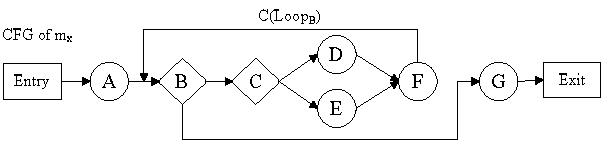
\includegraphics[width=3.5in, height=1in]{performance/images/cfg-new.pdf}
	
	\caption{An Example Control Flow Graph}	
	
	\label{fig:cfg-sample}
\end{figure}


%Ifwe try to estimate $freq(A, B)$ as a function of average iterations in $A$

%Generally, a change set may introduce performance regression in two ways: one case is the change itself in the hot path of execution and another case is that changes modifies some control variables which result some part of code executing very frequently. We can estimate how frequently the method executing in two ways: Loop correlation and Collection propagation. %Generally the changes inside a method does not lie in a single execution path. Control flow analysis of a modified method helps to identify all the paths inside the method and the changes in the path. 

   
\begin{multline}
\label{equa:example}
fq(m_x), m_y)=fq(A, m_y) + (Max(fq(D, m_y), fq(E, m_y))\\ + fq(F, m_y)) \times C(Loop_B) + fq(G, m_y)
\end{multline}
\vspace{-0.5cm}

%shown a simple CFG of a change of a modified method where each node represents a block of CFG and each annotated with cost which is sum of all the method execution time inside the block. There are two path from node B to node F.  $Cost\textsubscript{BDF}$ is the cost of path $BCDF$ and $Cost\textsubscript{BEF}$ is the cost of path $BCEF$. So the maximum cost will the maximum of this two path multiplied by the loop counter which is the execution time of changes in the method.


 
%\subsection{How to decide How many times a method will execute}
%Generally, a change set may introduce performance regression in two ways: one case is the change itself in the
%hot path of execution and another case is that changes modifies some control %variables which result some part of code
%executing very frequently. We can estimate how frequently the method executing in two ways: Loop correlation and Collection propagation.  

\subsection{Loop-Count Estimation with Collection-Loop Correlation} 

With the estimation of invocation frequency, the only remaining unknown parameter in the performance model of the new version is the loop count of all loops. If a loop exists in the base version and is not affected by the code commit, we directly use the recorded profile from the base version to acquire the iteration count. Two more complicated cases are (1) when a new loop is added, and (2) when the code commit affects the iteration count of an existing loop. Here is our insight: for collection-intensive software, we can construct the correlation between collection sizes and loop counts, and use iteration counts of known loops to infer that of unknown loops, as well as a code commit's impact on iteration counts of known loops. 

\subsubsection{Correlating Loops and Collections} In particular, we consider the following two types of dependencies between loops and collection variables:

\begin{itemize}
	\item Iteration Dependency. A loop $L$ is iteration-dependent on a collection variable $v$ if $L$'s loop condition depends on the size attribute of $v$.
	\item Operation Dependency. A collection variable $v$ is operation-dependent on a loop $L$ if there exists an element addition or removal on $v$ in $L$.
	\vspace{-0.15cm}
\end{itemize}

To identify iteration dependencies, for a For-Each loop (e.g, \CodeIn{for(A a : ListOfA)}), we simply consider that the loop is iteration-dependent on the collection variable being iterated via the loop. For other loops, we use standard inter-procedural data flow analysis~\cite{SootIFDS}~\cite{IFDS} to track data dependency backward from the loop condition expression, until we reach a size/length attribute of an array or a known collection class from the Java Collection Library. To make sure that the collection size is comparable with the loop count, we consider only two types of data dependencies: (1) direct assignment (e.g., \CodeIn{a = b;}), and (2) addition or subtraction expression with one operand as constant (e.g., \CodeIn{a = b.size() - 1}). 

To identify operation dependencies, for each loop $L$, we check its body for element-addition and element-removal operations on collection variables. For any other method invocations in the loop, we recursively go into the body of each invoked method to further look for such operations. However, we do not consider nested-loop blocks in $L$ or a method invoked from $L$, because such blocks are dependent on their direct enclosing loop. For example, in Figure~\ref{fig:operationDepend}, collection variable $v$ is operation-dependent on Loop$_A$, but $w$ is not (it is operation-dependent on Loop$_B$). 

\begin{figure}
\centering
	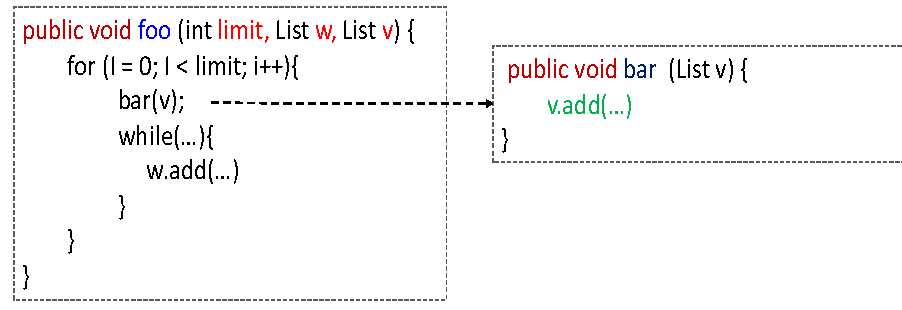
\includegraphics[width=3.5in, height=1.3in]{performance/images/operationDepend.pdf}
	
	\caption{Code Sample of Operation Dependency}	
		
	\label{fig:operationDepend}
\end{figure}




After identifying these two types of dependency relations, we further apply points-to analysis~\cite{Spark} to identify alias relations among collection variables. Note that in our analyses we consider only variables of known collection classes from the Java Collection Library. User-defined collections are also common. However, since we use inter-procedural analysis for identifying both types of dependencies, as long as the user-defined collections extend or wrap Java-Collection classes from the Java Collection Library, we are able to handle these user-defined collections by building dependencies directly on the Java-Collection variables inside them. Also note that  we identify all dependencies and alias relations on the base version and record the results so that we need to re-analyze only the revised/added methods when a code commit comes. 

\vspace{-0.2cm}
\subsubsection{Iteration-Count Inference}


With the dependencies identified among collections and loops, when a new code commit comes, we use Algorithm~\ref{alg:infer} to infer the iteration count of new loops and update the iteration count of existing affected loops. 

In the algorithm, we use a work queue to iteratively update sizes of collection variables and loop-iteration counts (stored in $lCount$), and we use the combined map of $MapI$ and $MapO$ to transit between collections and loops. In particular, as shown in Lines 6-11, we update the iteration count of each loop at most once, to avoid infinite update process caused by cyclic dependency (the more in-depth reason is that we use numbers to represent iteration counts, which are not in a bounded domain). In the end, we remove collection variables from $lCount$ to retain only the loops in the map.

\setlength{\textfloatsep}{6pt}
\begin{algorithm}[t]
	\begin{algorithmic}[1]		
		\REQUIRE~~\\
		$MapO$ is a map from collection variables to loops\\
		$MapI$ is a map from loops to collection variables\\
		$lCount$ is a map from loops to iteration counts\\
		\ENSURE~~\\ updated $lCount$\\
		\STATE{$Q \leftarrow MapI.keys()$}
		\STATE{$Map \leftarrow MapO \bigcup MapI$}
		\WHILE{$Q \neq \emptyset$}
		\STATE{$top \leftarrow Q.pop()$}
		\FORALL{$val \in Map.get(top)$}
		\IF{$val \notin lCount.keys() $}
		\STATE{$lCount.add(val, lCount.get(top)$}
		\STATE{$Q.add(val)$}
		\ELSIF{$val$ is a collection variable}
		\STATE{$lCount.set(val, lCount.get(val) + lCount.get(top)$}
		\STATE{$Q.add(val)$}
		\ENDIF
		\ENDFOR
		\ENDWHILE
		\STATE{$lCount.removeAll(MapO.keys())$}
	\end{algorithmic}
	\caption{Iteration Count Inference}
	\label{alg:infer}
\end{algorithm}

\vspace{-0.2cm}
\subsection{Test Case Prioritization}
\vspace{-0.1cm}
Once our approach estimates the performance impact of the code commit on each test case, we can rank test cases according to their relative performance impact. We use the main method as the root for system tests and each test method as the root for unit tests. We consider both positive and negative effect on execute time as it is often also important for developers to understand whether and where their commit is able to enhance the software performance. 


%In the figure ~\ref{fig:approach_overviw_1}, changes in the method named as getNameSpaceURI is trivial to developer because the indirect cost is not visible to developer. We can see that grand parent in the calling stack has loop in nested which execute more that 8000 time in both case. As a result the changes happen in hot path introduce high cost. Furthermore, developer may not be aware of another loop in path which is a child method in calling stack. As a result average counter of this loop in each test case more than 144000 times which introduce performance regression. To address this problem we introduce call graph with calling context that will provide estimation how many times the modified method getNameSpaceURI could be called from parent. if we know the frequency of the method getNameSpaceURI in the context then it is easy to say how many time the newly added method will be invoked. Similarly the newly added child has a loop that correlated with array size provide the context how many time the methods inside loop will be executed. 

%\begin{figure}
%  \centering
%  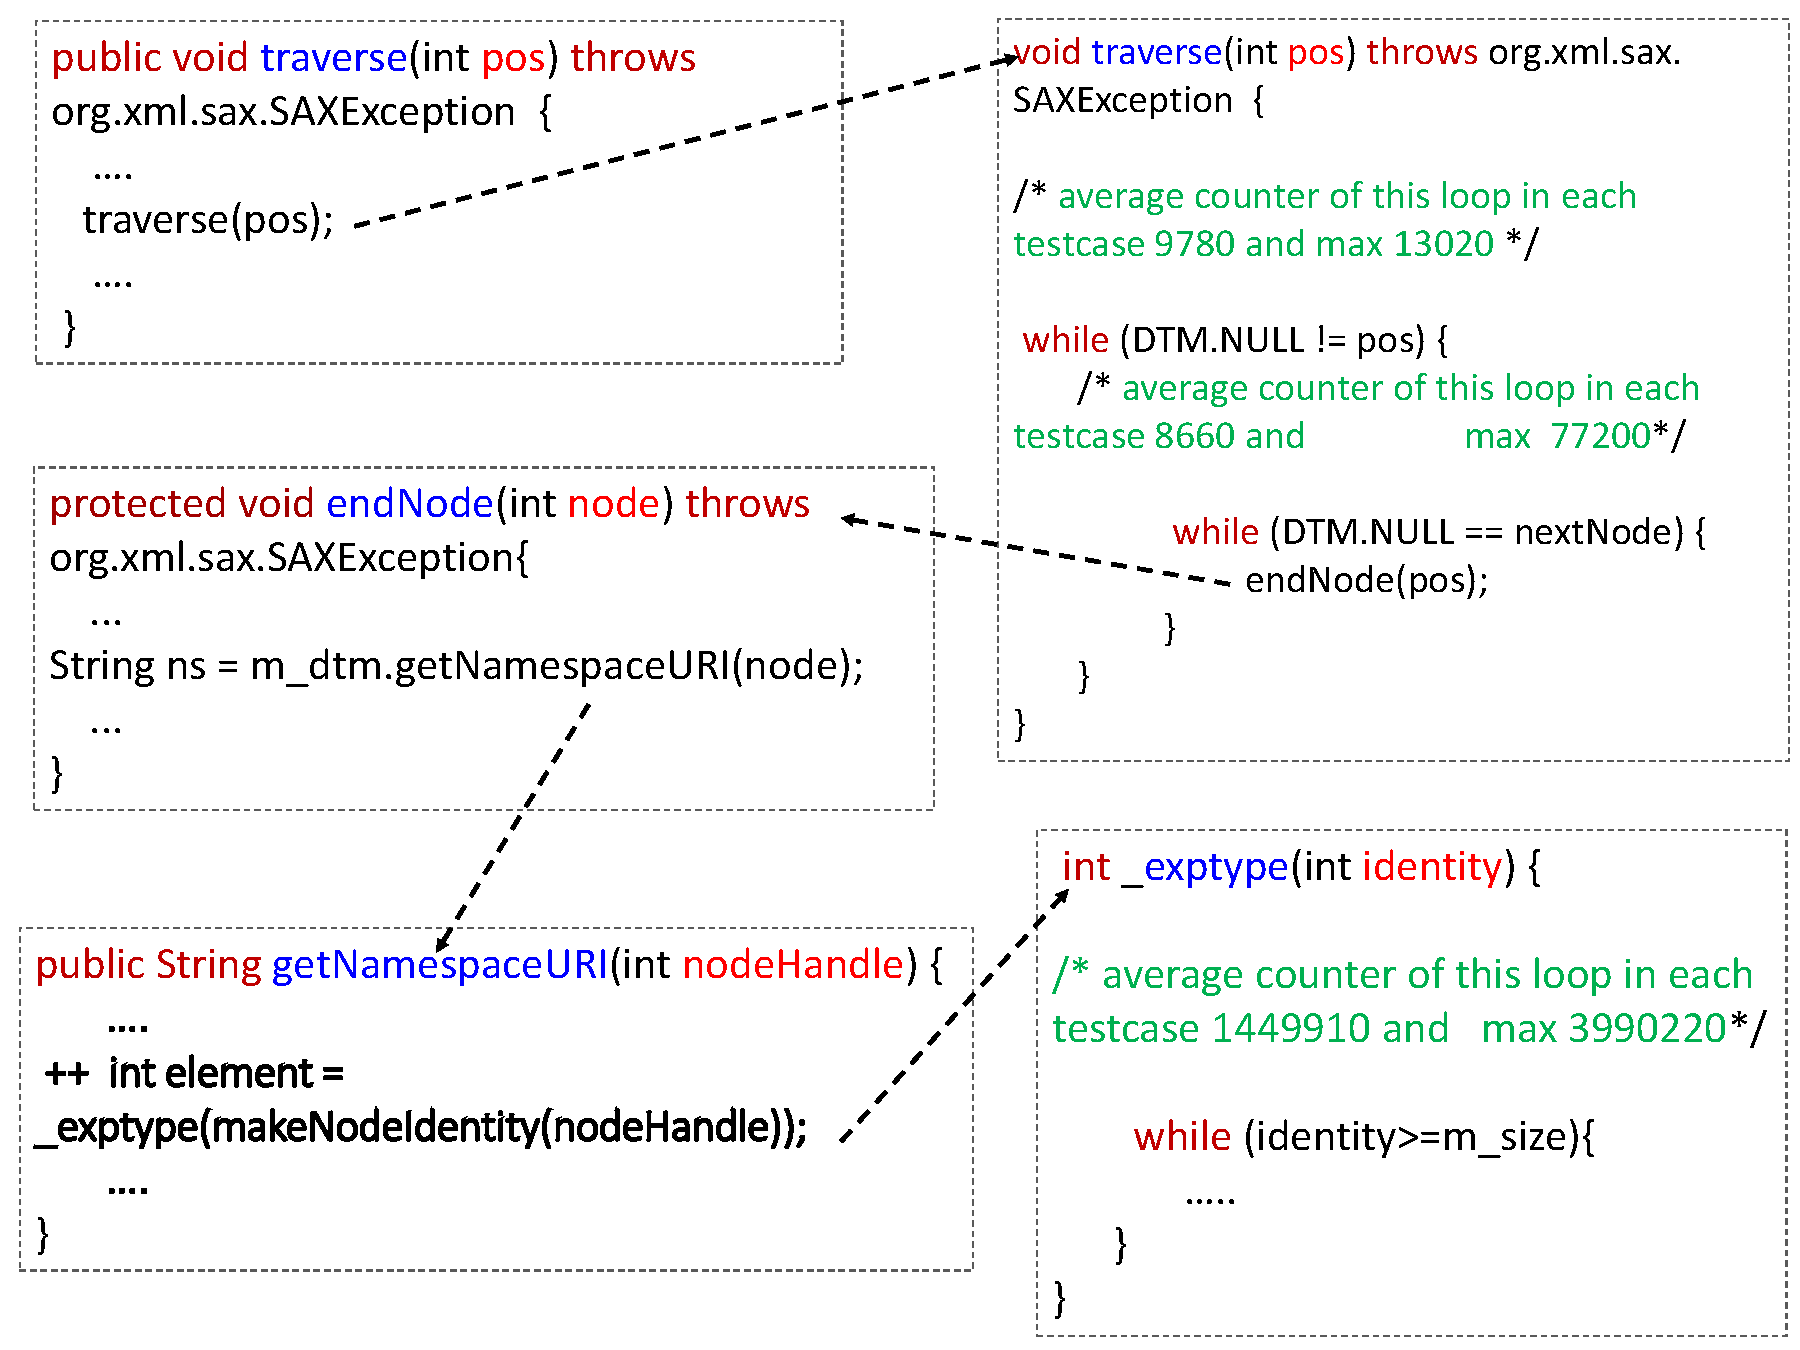
\includegraphics[width=\columnwidth,height=3in]{images/call-graph-example.pdf}
%  \caption{Overview of a change call graph in Xalan}	
%  \label{fig:approach_overviw_1}
%\end{figure}

%\subsubsection{Collection Propagation}
%The most common nature of loop in source code is iterate of over array or collections and changes inside loop introduce cost. 
%Generally, collection or array are propagated two ways: parameter passing and field variable. In the figure ~\ref{fig:approach_overviw_2} we can see that three different methods has loop that depends on the size of ArrayList and most
%importantly they are alias. if one of method loop counter is known then any new invocation of other method's loop counter can be predicted which will be helpful to estimate how many times the method under a loop will be called. So static analysis and alias analysis are important way to the solution of the problem.
%
%\begin{figure}
% \centering
%  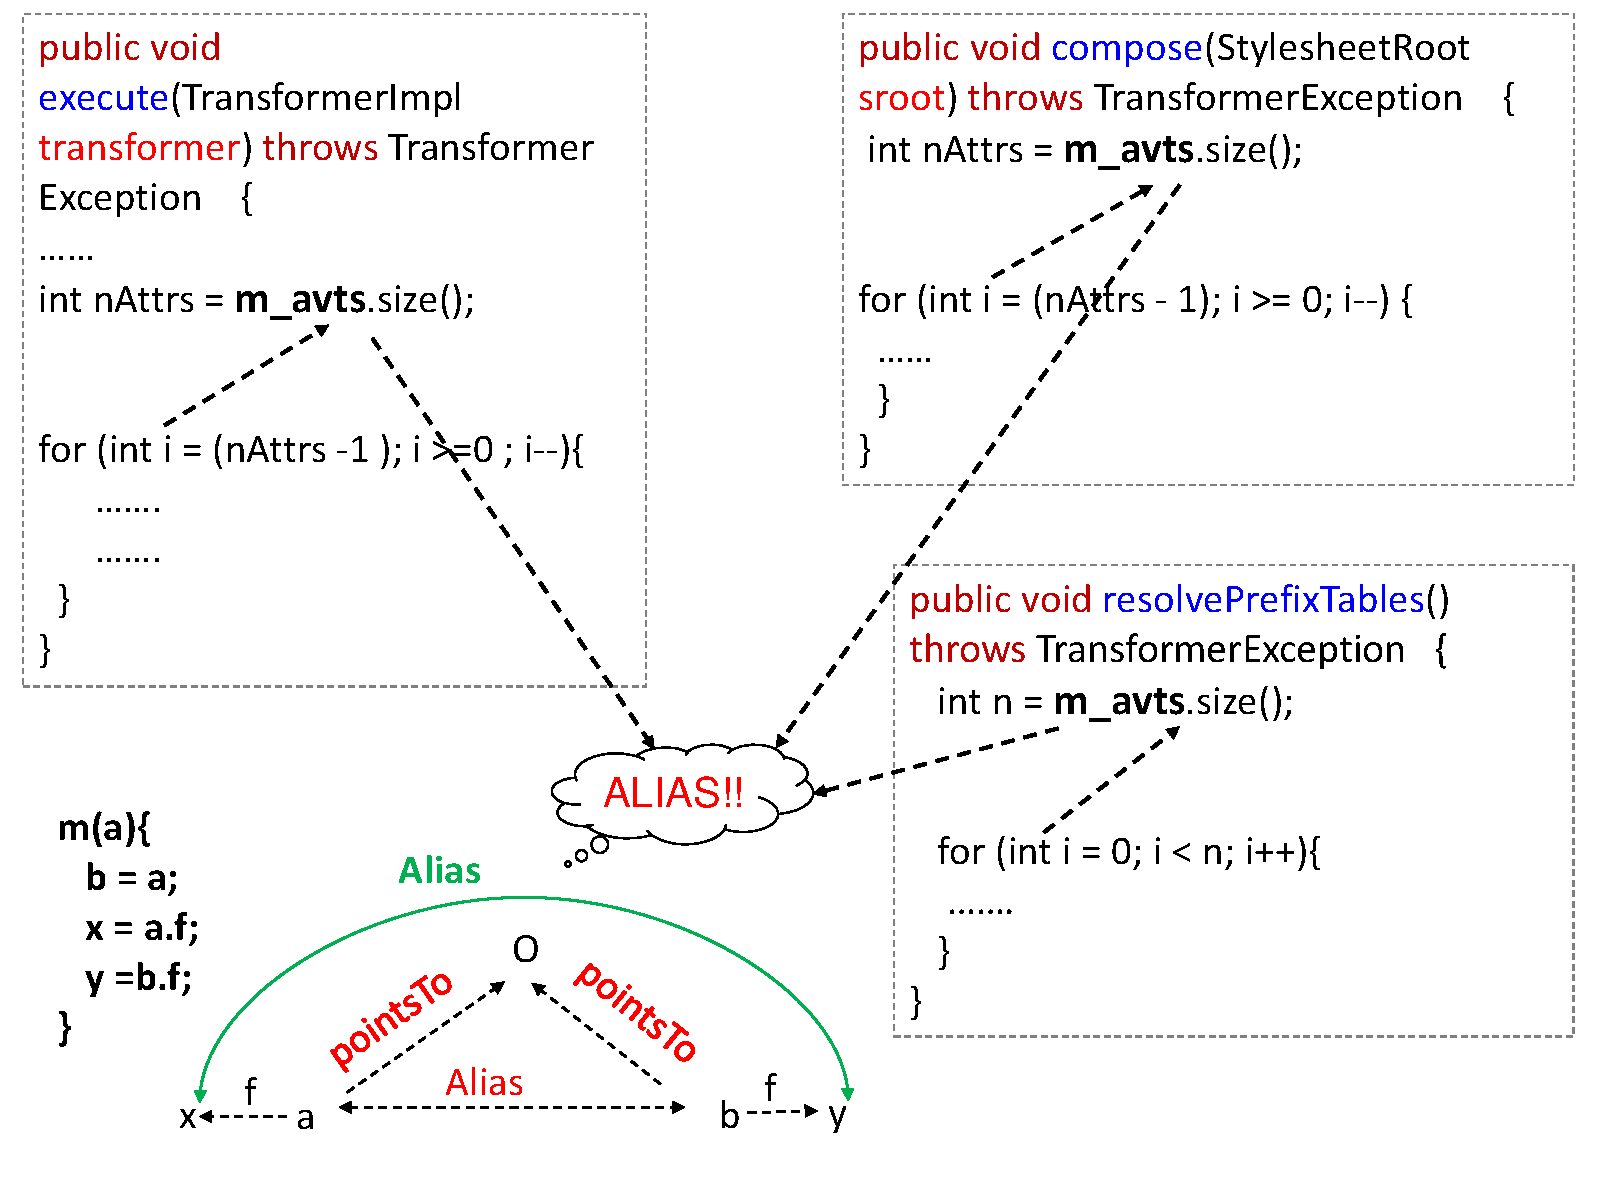
\includegraphics[width=\columnwidth,height=3in]{images/Alias-example.pdf}
%	\caption{Overview of a alias in Xalan}	  
%  \label{fig:approach_overviw_2}
%\end{figure}
%
%
%\begin{algorithm}
%\SetAlgoLined
%\SetKwInOut{Input}{Input}\SetKwInOut{Output}{Output}
%
%\Input{git version1 head and version2 head}
%\Output{List Added, List Deleted}
%
%\BlankLine
%
%$fileDiff$ = git diff [--options] version1 version2\;
%$listDiff$ = Diffparser($fileDiff$)\;
%$listDiff$ = Filter($listDiff$)\;
%$listAdded$ =[] \;
%$listDeleted$ =[] \;
%\ForEach{each diff $d$ in $listDiff$}{
%  
%	\uIf{$added$}{
%  add tuple $<$class, method, startLine, endLine$>$ to $listAdded$\;
%	}\uElseIf{$deletd$}{
%   add tuple $<$class, method, startLine, endLine$>$ to $listDeleted$\;
%  }\Else{
%    do nothing\;  
%  }
%
%}
%
%\Return{[$listAdded$,$listDeleted$]}
%
%\caption{Change List Generation}
%\label{alg:the_alg_1}
%\end{algorithm}
%
%
%\begin{algorithm}
%\SetAlgoLined
%\SetKwInOut{Input}{Input}\SetKwInOut{Output}{Output}
%
%\Input{$listAdded$,$listDeleted$}
%\Output{Rank of Test suite}
%
%\BlankLine
%
%$listTest$ = getAllTestSuite()\;
%$globalSummary$ = GlobalSummary()\;
%$mapCost$ = $<$test$,$cost$>$ \;
%\ForEach{each Test $t$ in $listTest$}{
%
%  $callGraph$ = LoadCallGraph($t$)\;
%  $localSummary$ = LocalSummary($t$)\;
%  $loopCounter$ = LoopCounter($t$)\;
%	$cost$ = 0;\;
%	
%	\uIf{$listAdded$ contain in $callGraph$}{
%	     buildCFG($listAdded$)\;
%	     cost += estimate addition cost of change from loop counter, local and global method execution summary\;       
%	}\uElseIf{$listDeleted$ contain in $callGraph$}{
%	     buildCFG($listDeleted$)\;
%       cost -= estimate deletion cost of change from loop counter, local and global method execution summary\;     
%	}\Else{
%    do nothing\;  
%  }
%  
%  update $mapCost$\;
%
%}
%
%$mapScore$ = $<$test$,$score$>$ \;
%\ForEach{each Test $t$ in $mapCost$}{
%   
%   $score$ = ($oldTime$ + $cost$)/ $oldTime$ \;
%   update $mapScore$\;
%    
%}
%
%
%$rankedList$ = runRankingAlgo($mapScore$)\;
%
%\Return{[rankedList]}
%
%\caption{Change Impact Performance Analysis}
%\label{alg:the_alg_2}
%\end{algorithm}

%\subsection{Collection-aware Performance Impact Analysis}
%
%Our change impact performance analysis algorithm \ref{alg:the_alg} takes two git head version of source code and automatically generate
%the diff between the two version. Statically analyse the generated diff and extract the list of methods added and deleted in the change source code with start and end line of a change inside a method. In the figure \ref{fig:approach-overviw-3} a modified method simple 
%CFG is shown. Maximum path among the two path is multiplied by loop counter consider as the cost impact. For each test case we calculate total impact cost according to the algorithm form line 17 to 30. Finally return the ranked list of test suite on the basis of
%performance impact. The figure \ref{fig:approach-workflow} describe the complete workflow of our approach.
%
%Our approach divided into two stage: generate change list and change impact analysis. Our change list generation algorithm\ref{alg:the_alg_1} takes two git head version of source code and automatically generate the diff between the two version. From line 1 to 3 describe the process of diff generation, parsing and filtering. First it statically analyse the generated diff contain and filter out the insignificant changes and other non non-relevant changes like java doc, comments etc. From line 6 to 14 describe the process of   extracting list of methods added and deleted in the change source code with start and end line number of a change inside a method. Finally return the list of algorithm\ref{alg:the_alg_1} feed to Our change impact analysis algorithm\ref{alg:the_alg_2}.
%From line 4 to 19 it describe the process of change list impact estimation. To estimating the cost it first build CFG of change method and find out the changes in the path of CFG. Then assign cost to each of the block from profile database which is describe in the figure \ref{fig:approach-overviw-3}. After estimating the cost of a method change, total impact of cost is calculated from the call graph which is  describe in the figure \ref{fig:performance-model}.Finally line 20 to 26 describe the return the ranked list of test suite on the basis of performance impact score.
% 
